\chapter{Locally-linear pictorial structures}
Human pose estimation from single, 2D images holds great potential to assist in 
a wide range of applications---semantic indexing of images and videos, action 
recognition, activity analysis, and human computer interaction, to name a few.
However, human pose estimation ``in the wild'' is an extremely challenging 
problem.  It shares all of the difficulties of object detection, such as 
confounding background clutter, lighting, viewpoint, and scale, in addition to
significant difficulties unique to human poses.  There is an enormous 
variation in foreground color and texture due to clothing, and even given 
viewpoint and pose, the shape of body parts is highly variable due to clothing, 
relative scale variations, and articulation (causing foreshortening, 
self-occlusion and physically different body contours).

\begin{figure}[t!]
\centering
\includegraphics[width=0.99\linewidth]{data/model-overview.pdf}
\caption{\small \label{fig:overview} \textbf{Left:} Most pictorial structures 
researchers have put effort into better and larger feature spaces, in which 
they fit one linear model.  The feature computation is expensive, and we still 
fail at capturing the many appearance modes in real data.  \textbf{Right:} We 
take a different approach.  Rather than introduce more and more features in 
hopes of high-dimensional linear separability, we model the non-linearities in 
simpler, lower dimensional feature spaces, using a collection of {\em locally} 
linear models.}
\end{figure}


As a motivating example, consider the multitude of variations of left elbows, 
ignoring color and lighting variations.  First, consider the range of body 
types---infant elbows and adult elbows, male elbows and female elbows, fat 
elbows and skinny---a conservative estimate would say there are 5 coarse body 
type modes.  Considering clothing, there are baggy long sleeves, tight long 
sleeves, stripes, solids, bare arms, and short sleeves ending near the 
elbow---let's assume we can summarize clothing variation around elbows with 5 
appearance modes (also overly optimistic).  Finally, given body type and 
clothing, we still must consider articulation.  A typical discretization of 
angles to model human pose~\cite{felzps,devacrf,eichner09,sapp2010cascades} 
uses $15^\circ$ increments for a total of 24 possible relative angles.  As a 
rough back-of-the-envelope calculation, this already amounts to $5 \times 5 
\times 24 = 600$ major appearance modes, just for the elbow.  See 
Figure~\ref{fig:lelbs} for an illustration.

\begin{figure}[b!]
\centering
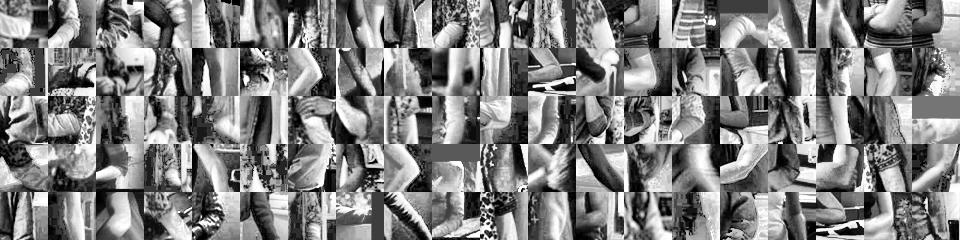
\includegraphics[width=0.99\linewidth]{data/lelbs.jpg}
\caption{\small \label{fig:lelbs} A random sampling of 100 left elbows from the 
Buffy Stickmen pose dataset, removing color and intensity bias, to illustrate 
the huge variety of appearance due to clutter, motion blur, clothing, body 
type, and pose.}
\end{figure}

Clearly, some degree of sharing between appearance modes is warranted and 
beneficial, in particular because it is easier to estimate fewer model 
parameters.  However, most models developed for this problem take sharing to an 
extreme, and use {\em just a single, linear 
model}~\cite{devacrf,eichner09,sapp2010cascades,sapp2011,andriluka09,ddtran}.  
Such models make it very difficult to capture the part variations discussed.  
Most researchers focus attention on improving features in hopes that a better 
feature space will make a linear model work.  Only recently, several papers 
studied increasing the number of modes in pose models. However, these works 
used at most only tens of modes per part, and struggle with discovery of latent 
modes and/or defining an effective discrete quantization of the pose space.  
See Section~\ref{sec:rel} for details.


\mypar{Our approach:} In this paper, we propose a model of human pose that 
defines a mode {\em per training example}, to capture a local neighborhood of
pose {\em and } appearance.  This results in hundreds or thousands of modes in 
contrast to the 20 or fewer used by recent work. This gives us the ability to 
precisely model pose and appearance using a linear, structured model for each 
local neighborhood.  Because of this defining characteristic, we call our model 
\model~(\mdl).

We define the extent of each neighborhood in terms of radii in appearance and 
pose, which decompose at a part level.  As a result, the training example space 
is well covered, and we have overlap between modes.  This allows us to heavily 
share training data and gives us a smoothly varying representation of the space 
of 2D human poses.

Using our explicit formulation of locality, no latent modes need to estimated, 
and no decisions made as to quantization degree and mode placement.  We propose 
a simple convex max-margin learning objective to fit parameters of our model.  
We show our model is competitive with state-of-the-art approaches from this 
year, while employing only very simple features. Further, inference is cheap 
and heavily parallelizable, taking only a few seconds per image.


\section{Modeling}\label{sec:model}
As discussed, due to the intractability of jointly tracking multiple objects through time, previous 
work has made limiting assumptions in both the representation of pose (i.e., 
the inability to model foreshortening or fine angular granularity), and the 
interactions between parts, which do not capture rich, image-dependent 
relationships.  We address each of these issues in a principled framework.

\subsection{Stretchable models of human pose}  One of the biggest limitations 
of current models of human pose is the ``cardboard people'' 
assumption~\cite{cardboard02}: that body parts are rigid patches of fixed size 
(up to a global scale).  In the Pictorial Structures (PS) framework~\cite{felzps}, the human is represented as a collection of parts with fixed lengths, 
which along with the position and angle of each joint, completely determines 
the pose of the person~\footnote{The seminal work of Felzenswalb et 
al.~\cite{felzps} uses 10 discretized scales per part, 
but all modern implementations of PS use one fixed scale~\cite{sapp2010cascades,ferrari08,andriluka09}, partly due to its prohibitive 
increase in the state space.}.  Thus, wrists are always a fixed distance away 
from elbows in these models. This is a frequently violated assumption in 
realistic video, due to foreshortening and variation in body type.  In the VideoPose2.0 dataset we  
introduce (Section~\ref{sec:experiments}), 30\% of lower arms 
are significantly foreshortened.

\mypar{Two joints $>$ one limb:} Rather than model human limbs as a position 
and orientation, we propose a model {\em directly on the pixel coordinates of 
each joint}.  Although this choice introduces more variables 
(one for each joint rather than for each part), the state space for each 
variable is drastically reduced because we no longer need to reason over a 
finely discretized set of angles in the state space, and we can now implicitly 
represent nearly any angle between parts.  In current PS implementations, this is a 
$24\times$ reduction in the state space of each variable.  In addition to 
this, because the length of the limb is now determined implicitly by the pixel 
distance between neighboring joints, the model naturally lends itself to 
capturing large variability in the part length.  Because of its ability to 
represent finely discretized limb length, we refer to this model as
{\em stretchable}, in contrast to the typical rigid, rectangle-based 
representation.

One side-effect of switching from a limb-centric to joint-centric model of 
pose is that unary attributes of the limb-centric model are now pairwise 
attributes of a joint-centric model.  Furthermore, pairwise attributes in a 
limb-centric model correspond to ternary attributes in a joint-centric model, 
which we do not use.  However, in a standard PS model, pairwise attributes are 
only image-independent functions of geometry, whereas in our model, pairwise 
potentials all incorporate image information, giving us overall a more 
expressive model than standard PS. 



\subsection{Structured Ensemble of Stretchable Models}
Ideally we want a model of human motion which captures important
relationships between all correlated parts.  This includes parts that
are connected kinematically (e.g., left elbow, left wrist), parts that
are left/right symmetric (e.g., left elbow, right elbow), and
instantiations of the same part in consecutive frames (e.g., left
elbow at time $t$, left elbow at time $t+1$).  Clearly, modeling all
these relationships together leads to cyclic dependencies
within a single frame (due to the three symmetry edges) and
between consecutive frames (due to the six tracking edges); see Figure~\ref{fig:overview}, left. 

However, in general, it is always possible to express the score of a
given state assignment in a full, intractable model as the sum of
scores under a set of tree sub-models that collectively cover every
edge in the full model. This is the key insight that allows us to
include all the rich relationships we desire: we {\em decompose} our
model of all interesting relationships related to parsing human motion
into an ensemble of submodels, all of which are trees (and therefore
tractable). Each tree submodel is responsible for tracking a single
joint through time and additionally models the corresponding set of
pairwise interactions between joints in a single frame
(Figure~\ref{fig:overview}, right).

\subsection{Formulation}
Formally, we pose this problem as a structured prediction task, where
the input $x$ is a video sequence of $\ell$ images and the output $y$ is a
sequence of $P\ell$ variables, where $P$ is the number of parts (joint
locations) included in the model. Each output $y_i$ is the 2-D
coordinate of some part joint (defined in a $80 \times 80$
discretization of the pixel space) in some frame.  We also use the shortcut notation 
$y_{\bf t} = \{ y_i \;|\; y_i \text{ is in frame } t \}$
to index all $P$ joint variables in frame $t$. Given a training set
$S = \{\ang{x^{(j)},y^{(j)}}\}_{j=1}^n$ of samples from a joint
distribution, the standard supervised learning task is to learn a
hypothesis $h: X \mapsto Y$ that minimizes the expected loss $\E{S}{
  \cL\left(h(x^{(j)}) , y^{(j)}\right)}$ for some non-negative loss function $\cL
: Y \times Y \rightarrow \reals^+$. The linear hypothesis class we
consider is of the form $h(x) = \argmax_y \score{y}$, where the
scoring function $\score{y} \triangleq \theta^\top \bft(x,y)$ is the
inner product of a vector of parameters $\theta$ and a feature
function $\bft: X \times Y \mapsto \reals^d$ mapping $(x,y)$ pairs to
$d$ real-valued features. Let $G = (\cV,\cE)$ be our full graphical
pose model; we further assume that $\bft$ decomposes over the vertices
$\cV$ and edges $\cE$, so that
\begin{equation}
  \label{eq:model-score}
  \score{y} = \sum_{(i,j) \in \mcal{E}}\theta^\top\bft_{ij}(x,y_i,y_j) +
  \sum_{i \in \mcal{V}}\theta^\top\bft_i(x,y_i).
\end{equation}
Note that edges $(i,j)$ may connect variables between consecutive
frames. Let there be $M$ tree sub-models, and $G_m = (\cV, \cE_m)$ be the sub-graph of $G$ corresponding
to the $m$'th one as in Figure~\ref{fig:overview}, right.  Then
we decompose the score $\score{y}$ into the sum of the scores of the
$M$ constituent sub-models: $\score{y} = \sum_{m=1}^M \pscore{y}$, the
score of the $m$'th model is as in Equation~\ref{eq:model-score}, restricted to the
edges $\cE_m$, i.e. $\pscore{y} =
\sum_{(i,j)\in\cE_m}\theta_m^\top\bft_{ij}(x,y_i,y_j) +
\sum_{i\in\cV}\theta_m^\top\bft_i(x,y_i)$. Note that we do not couple
parameters across different models $\theta_m$.

\out{
\begin{figure}[]
\centering
\includegraphics[width=0.9\linewidth]{figs/dd_vs_sub.pdf}
\caption{\small \label{fig:dd} Decoding with Dual Decomposition
  (examples). \textbf{Left:} The argmax predictions of each of the
  sub-models in the ensemble; note the disparity in predictions.
  \textbf{Right:} The prediction after running Dual Decomposition for
  500 iterations or until convergence (Yellow) compared to the
  predictions from \cite{sapp2010cascades} (Magenta).}
\end{figure}
}

\subsection{Structured Model Inference}
We explore several methods for combining the $M$ independent models
during test time to make a single final decision.  The methods form a
hierarchy of agreement criteria between the submodels: at one extreme,
we enforce the constraint that all submodels must agree on the
maximizing assignment to all variables, and at the other, inference is
completely decoupled across submodels. Note that there is an inherent
trade-off between the degree of agreement imposed on the models and the
computational cost of the corresponding inference.  We present our
inference methods by order of decreasing agreement below.

\paragraph{Full Agreement via Dual Decomposition.} A natural goal is
to find the argmax decoding of joint locations throughout the entire
sequence of frames using our original model in
Eq.~\ref{eq:model-score}. However, solving the argmax decoding problem
exactly is prohibitively expensive, due to the high treewidth of this
cyclic graph. We use the method of Dual Decomposition (DD)
\cite{bertsekas99,komodakis2007dualdecomp} to solve a linear
programming relaxation of the decoding problem as follows. Observe
that the argmax decoding problem of our full model can be decomposed
into $M$ sub-problems { if those problems are coupled through a global
  equality constraint}:
\begin{align}
  \label{eq:dual-decomp}
&\argmax_{y, y^1,\dots,y^m} \sum_{m=1}^M \pscore{y^m}  \textrm{ s.t. } \:  y^m=y  \quad{}\quad{(DD)}
\end{align}
Although the optimization \eqref{eq:dual-decomp} is still intractable because of the integral constraints, optimizing the {\em dual} of \eqref{eq:dual-decomp} is always
tractable (if we first drop the integrality requirement), but no longer guaranteed to return an optimal integral solution. We solve the dual problem with sub-gradient descent. Once complete agreement between all
$y^m$ is reached, then inference has converged to the exact solution
of \eqref{eq:dual-decomp} (although eventual convergence is not
guaranteed.) In our experiments, if dual decomposition did not
converge (after 500 iterations in practice, each requiring inference in all $M$ models), we used the maximum scoring primal variables found during
any descent iteration.

\out{To
solve the dual problem with sub-gradient descent, we introduce
Lagrange multipliers $\nu_{ik}^p$ for every possible state assignment
$y_i = k$ in every part model. We then alternate between updating the
dual variables $\nu^p$ and the primal variables $y^p$:
\begin{align}
  y^p & \leftarrow \argmax_y \left( \pscore{y} +  \sum_{i,k} \nu^p_{ik} \ind{y_i=k^p}\right) \\
  \nu^p_{ik} & \leftarrow \nu_{ik} - \alpha\left(  \ind{y_i^p=k} - \frac{1}{P}\sum_p \ind{y_i^p=k} \right),
\end{align}
where $\ind{\cdot}$ is the indicator function and $\alpha$ is a rate
parameter chosen according to the scheme given in
\cite{komodakis2007dualdecomp}.
} 


\paragraph{Single Frame Agreement.} An alternative to computing the
MAP decoding of the entire sequence is to find the argmax solution
while constraining model agreement to only a subset of the variables
at a time.  If we restrict our attention to the variables in a single
time frame only, inference is considerably simpler.  For each frame
$t$, we solve
\begin{equation}
\argmax_{y_{\bf{t}}'} \sum_{m=1}^M \max_{y : y_{\bf{t}} = y_{\bf{t}}'} \pscore{y} \quad{}\quad{(SF)}
\end{equation}
to obtain the joint configuration for that frame (remember $y_{\bf t}$
denotes the {\em set} of P joint variables in frame $t$).  In words,
the inner maximization finds the highest scoring sequence $y$ subject to
the constraint that the variables in frame $t$ are fixed at positions
$y_{\bf t}'$.  The outer argmax is over all possibilities of single
frame configurations $y_{\bf t}'$.  This extends the notion of a
max-marginal of a variable (see ~\cite{weiss10}) to a max-marginal
over {\em a set} of variables.  This method requires first computing
the max-product messages sent to variables in frame $t$, in each of
the submodels.  Finding the argmax decoding of $y_{\bf t}$ is then
equivalent to inference in a grid with P variables (in our case $P=6$
joints).  This can be solved exactly by forming cliques of size 3, for
which the message passing clique-tree forms a chain.  In each clique,
there are at most pairwise potentials, and since the state space of
each part is relatively small ($|Y_p| \leq 500$), the $O(\sum_p
|Y_p|^3)$ cost of this inference takes less than a second per frame in
practice, and in our experiments took about as long as performing inference in all $M$ tree submodels (i.e., twice as slow overall).


\paragraph{Single Variable Agreement.} 

We can further narrow our subset of interest down to a single variable
at a time \cite{weisssapp10}.  This is a weaker criteria for model
agreement, but yields cheaper and simpler inference.  This gives us
the following inference problem for the $i^{th}$ variable:
\begin{equation}
\argmax_{y_i'} \sum_{m=1}^M \max_{y: y_i=y_i'}\pscore{y} \quad{}\quad{(SV)}
\end{equation}
This can be solved by computing max-marginals for each model using standard forward-backward message passing, summing the $M$ max-marginal scores, and taking the highest scoring sum.
Note that this is actually equal to MAP decoding in the full model when  
all sub-models agree on the argmax, which rarely occurs in practice. However, in \cite{weisssapp10} we showed
empirically that this decoding is a useful approximation
of the full MAP decoding prediction. 

We also compared the above methods to predicting each joint using the single model in
the ensemble that incorporated temporal dependencies for that
specific part, which we call the $Independent$ decoding scheme.


\subsection{Learning} Although we enforce agreement during ensemble inference 
at {\em test time}, coupling inference during training for more than one 
variable is prohibitively expensive to use as part of a learning procedure.  
Thus we learn
parameters $\theta_m$ using {\em decoupled} inference separately for
each model. To learn parameters, we optimize a convex hinge-loss
objective for each model separately. Let $\pscoremaxj~=~\max_y~\pscorej{y}$ and $y^{\star(j)}$ a corresponding maximizer, then the learning problem is 
{\small
\begin{align*}
\min_{\theta_m} \frac{\lambda}{2}||\theta_m||^2 +
\frac{1}{n}\sum_{j=1}^n \left[ \pscoremaxj + \ind{y^{\star(j)} \neq y^{(j)}} - \pscorej{y^{(j)}}  \right]_+
\end{align*}}
where $[\cdot]_+ = \max(0,\cdot)$.
\out{
$\theta_m^\star =
\min_{\theta_m} \frac{\lambda}{2} ||\theta_m||^2 +
\frac{1}{n}\sum_{i=1}^n H(x^{(i)},y^{(i)},\theta_m)$, where $H$ is the hinge loss function, 
$H(x^{(i)},y^{(i)},\theta_m) = \left[ \pscorei{y^{i}} - \max_y \pscorei{y} - \ind{y\ne y^{(i)}} \right]_+$.
}
We optimize
this problem via stochastic sub-gradient descent, and we choose
$\lambda$ and the number of training epochs using a held-out
development set to minimize error.



